% ----------------------------------------------------------------------
%
%                            TFMTesis.tex
%
%----------------------------------------------------------------------
%
% Este fichero contiene el "documento maestro" del documento. Lo único
% que hace es configurar el entorno LaTeX e incluir los ficheros .tex
% que contienen cada sección.
%
%----------------------------------------------------------------------
%
% Los ficheros necesarios para este documento son:
%
%       TeXiS/* : ficheros de la plantilla TeXiS.
%       Cascaras/* : ficheros con las partes del documento que no
%          son capítulos ni apéndices (portada, agradecimientos, etc.)
%       Capitulos/*.tex : capítulos de la tesis
%       Apendices/*.tex: apéndices de la tesis
%       constantes.tex: constantes LaTeX
%       config.tex : configuración de la "compilación" del documento
%       guionado.tex : palabras con guiones
%
% Para la bibliografía, además, se necesitan:
%
%       *.bib : ficheros con la información de las referencias
%
% ---------------------------------------------------------------------

\documentclass[12pt,a4paper,twoside]{book}

%
% Definimos  el   comando  \compilaCapitulo,  que   luego  se  utiliza
% (opcionalmente) en config.tex. Quedaría  mejor si también se definiera
% en  ese fichero,  pero por  el modo  en el  que funciona  eso  no es
% posible. Puedes consultar la documentación de ese fichero para tener
% más  información. Definimos también  \compilaApendice, que  tiene el
% mismo  cometido, pero  que se  utiliza para  compilar  únicamente un
% apéndice.
%
%
% Si  queremos   compilar  solo   una  parte  del   documento  podemos
% especificar mediante  \includeonly{...} qué ficheros  son los únicos
% que queremos  que se incluyan.  Esto  es útil por  ejemplo para sólo
% compilar un capítulo.
%
% El problema es que todos aquellos  ficheros que NO estén en la lista
% NO   se  incluirán...  y   eso  también   afecta  a   ficheros  de
% la plantilla...
%
% Total,  que definimos  una constante  con los  ficheros  que siempre
% vamos a querer compilar  (aquellos relacionados con configuración) y
% luego definimos \compilaCapitulo.
\newcommand{\ficherosBasicosTeXiS}{%
TeXiS/TeXiS_pream,TeXiS/TeXiS_cab,TeXiS/TeXiS_bib,TeXiS/TeXiS_cover%
}
\newcommand{\ficherosBasicosTexto}{%
constantes,guionado,Cascaras/bibliografia,config%
}
\newcommand{\compilaCapitulo}[1]{%
\includeonly{\ficherosBasicosTeXiS,\ficherosBasicosTexto,Capitulos/#1}%
}

\newcommand{\compilaApendice}[1]{%
\includeonly{\ficherosBasicosTeXiS,\ficherosBasicosTexto,Apendices/#1}%
}

\newcommand{\appadm}{TakeOrderAdmin}
\newcommand{\appweb}{TakeOrder}
%- - - - - - - - - - - - - - - - - - - - - - - - - - - - - - - - - - -
%            Preámbulo del documento. Configuraciones varias
%- - - - - - - - - - - - - - - - - - - - - - - - - - - - - - - - - - -

% Define  el  tipo  de  compilación que  estamos  haciendo.   Contiene
% definiciones  de  constantes que  cambian  el  comportamiento de  la
% compilación. Debe incluirse antes del paquete TeXiS/TeXiS.sty
%---------------------------------------------------------------------
%
%                          config.tex
%
%---------------------------------------------------------------------
%
% Contiene la  definición de constantes  que determinan el modo  en el
% que se compilará el documento.
%
%---------------------------------------------------------------------
%
% En concreto, podemos  indicar si queremos "modo release",  en el que
% no  aparecerán  los  comentarios  (creados  mediante  \com{Texto}  o
% \comp{Texto}) ni los "por  hacer" (creados mediante \todo{Texto}), y
% sí aparecerán los índices. El modo "debug" (o mejor dicho en modo no
% "release" muestra los índices  (construirlos lleva tiempo y son poco
% útiles  salvo  para   la  versión  final),  pero  sí   el  resto  de
% anotaciones.
%
% Si se compila con LaTeX (no  con pdflatex) en modo Debug, también se
% muestran en una esquina de cada página las entradas (en el índice de
% palabras) que referencian  a dicha página (consulta TeXiS_pream.tex,
% en la parte referente a show).
%
% El soporte para  el índice de palabras en  TeXiS es embrionario, por
% lo  que no  asumas que  esto funcionará  correctamente.  Consulta la
% documentación al respecto en TeXiS_pream.tex.
%
%
% También  aquí configuramos  si queremos  o  no que  se incluyan  los
% acrónimos  en el  documento final  en la  versión release.  Para eso
% define (o no) la constante \acronimosEnRelease.
%
% Utilizando \compilaCapitulo{nombre}  podemos también especificar qué
% capítulo(s) queremos que se compilen. Si no se pone nada, se compila
% el documento  completo.  Si se pone, por  ejemplo, 01Introduccion se
% compilará únicamente el fichero Capitulos/01Introduccion.tex
%
% Para compilar varios  capítulos, se separan sus nombres  con comas y
% no se ponen espacios de separación.
%
% En realidad  la macro \compilaCapitulo  está definida en  el fichero
% principal tesis.tex.
%
%---------------------------------------------------------------------


% Comentar la línea si no se compila en modo release.
% TeXiS hará el resto.
% ¡¡¡Si cambias esto, haz un make clean antes de recompilar!!!
\def\release{1}


% Descomentar la linea si se quieren incluir los
% acrónimos en modo release (en modo debug
% no se incluirán nunca).
% ¡¡¡Si cambias esto, haz un make clean antes de recompilar!!!
%\def\acronimosEnRelease{1}


% Descomentar la línea para establecer el capítulo que queremos
% compilar

% \compilaCapitulo{01Introduccion}
% \compilaCapitulo{02EstructuraYGeneracion}
% \compilaCapitulo{03Edicion}
% \compilaCapitulo{04Imagenes}
% \compilaCapitulo{05Bibliografia}
% \compilaCapitulo{06Makefile}

% \compilaApendice{01AsiSeHizo}

% Variable local para emacs, para  que encuentre el fichero maestro de
% compilación y funcionen mejor algunas teclas rápidas de AucTeX
%%%
%%% Local Variables:
%%% mode: latex
%%% TeX-master: "./Tesis.tex"
%%% End:


% Paquete de la plantilla
\usepackage{TeXiS/TeXiS}

% Incluimos el fichero con comandos de constantes
%---------------------------------------------------------------------
%
%                          constantes.tex
%
%---------------------------------------------------------------------
%
% Fichero que  declara nuevos comandos LaTeX  sencillos realizados por
% comodidad en la escritura de determinadas palabras
%
%---------------------------------------------------------------------

%%%%%%%%%%%%%%%%%%%%%%%%%%%%%%%%%%%%%%%%%%%%%%%%%%%%%%%%%%%%%%%%%%%%%%
% Comando: 
%
%       \titulo
%
% Resultado: 
%
% Escribe el título del documento.
%%%%%%%%%%%%%%%%%%%%%%%%%%%%%%%%%%%%%%%%%%%%%%%%%%%%%%%%%%%%%%%%%%%%%%
\def\titulo{\textsc{TeXiS}: Una plantilla de \LaTeX\
  para Tesis y otros documentos}

%%%%%%%%%%%%%%%%%%%%%%%%%%%%%%%%%%%%%%%%%%%%%%%%%%%%%%%%%%%%%%%%%%%%%%
% Comando: 
%
%       \autor
%
% Resultado: 
%
% Escribe el autor del documento.
%%%%%%%%%%%%%%%%%%%%%%%%%%%%%%%%%%%%%%%%%%%%%%%%%%%%%%%%%%%%%%%%%%%%%%
\def\autor{Marco Antonio y Pedro Pablo G\'omez Mart\'in}

% Variable local para emacs, para  que encuentre el fichero maestro de
% compilación y funcionen mejor algunas teclas rápidas de AucTeX

%%%
%%% Local Variables:
%%% mode: latex
%%% TeX-master: "tesis.tex"
%%% End:


% Sacamos en el log de la compilación el copyright
%\typeout{Copyright Marco Antonio and Pedro Pablo Gomez Martin}

%
% "Metadatos" para el PDF
%
\ifpdf\hypersetup{%
    pdftitle = {\titulo},
    pdfsubject = {Plantilla de Tesis},
    pdfkeywords = {Plantilla, LaTeX, tesis, trabajo de
      investigación, trabajo de Master},
    pdfauthor = {\textcopyright\ \autor},
    pdfcreator = {\LaTeX\ con el paquete \flqq hyperref\frqq},
    pdfproducer = {pdfeTeX-0.\the\pdftexversion\pdftexrevision},
    }
    \pdfinfo{/CreationDate (\today)}
\fi


%- - - - - - - - - - - - - - - - - - - - - - - - - - - - - - - - - - -
%                        Documento
%- - - - - - - - - - - - - - - - - - - - - - - - - - - - - - - - - - -
\begin{document}

% Incluimos el  fichero de definición de guionado  de algunas palabras
% que LaTeX no ha dividido como debería
%----------------------------------------------------------------
%
%                          guionado.tex
%
%----------------------------------------------------------------
%
% Fichero con algunas divisiones de palabras que LaTeX no
% hace correctamente si no se le da alguna ayuda.
%
%----------------------------------------------------------------

\hyphenation{
% a
abs-trac-to
abs-trac-tos
abs-trac-ta
abs-trac-tas
ac-tua-do-res
a-gra-de-ci-mien-tos
ana-li-za-dor
an-te-rio-res
an-te-rior-men-te
apa-rien-cia
a-pro-pia-do
a-pro-pia-dos
a-pro-pia-da
a-pro-pia-das
a-pro-ve-cha-mien-to
a-que-llo
a-que-llos
a-que-lla
a-que-llas
a-sig-na-tu-ra
a-sig-na-tu-ras
a-so-cia-da
a-so-cia-das
a-so-cia-do
a-so-cia-dos
au-to-ma-ti-za-do
% b
batch
bi-blio-gra-fía
bi-blio-grá-fi-cas
bien
bo-rra-dor
boo-l-ean-expr
% c
ca-be-ce-ra
call-me-thod-ins-truc-tion
cas-te-lla-no
cir-cuns-tan-cia
cir-cuns-tan-cias
co-he-ren-te
co-he-ren-tes
co-he-ren-cia
co-li-bri
co-men-ta-rio
co-mer-cia-les
co-no-ci-mien-to
cons-cien-te
con-si-de-ra-ba
con-si-de-ra-mos
con-si-de-rar-se
cons-tan-te
cons-trucción
cons-tru-ye
cons-tru-ir-se
con-tro-le
co-rrec-ta-men-te
co-rres-pon-den
co-rres-pon-dien-te
co-rres-pon-dien-tes
co-ti-dia-na
co-ti-dia-no
crean
cris-ta-li-zan
cu-rri-cu-la
cu-rri-cu-lum
cu-rri-cu-lar
cu-rri-cu-la-res
% d
de-di-ca-do
de-di-ca-dos
de-di-ca-da
de-di-ca-das
de-rro-te-ro
de-rro-te-ros
de-sa-rro-llo
de-sa-rro-llos
de-sa-rro-lla-do
de-sa-rro-lla-dos
de-sa-rro-lla-da
de-sa-rro-lla-das
de-sa-rro-lla-dor
de-sa-rro-llar
des-cri-bi-re-mos
des-crip-ción
des-crip-cio-nes
des-cri-to
des-pués
de-ta-lla-do
de-ta-lla-dos
de-ta-lla-da
de-ta-lla-das
di-a-gra-ma
di-a-gra-mas
di-se-ños
dis-po-ner
dis-po-ni-bi-li-dad
do-cu-men-ta-da
do-cu-men-to
do-cu-men-tos
% e
edi-ta-do
e-du-ca-ti-vo
e-du-ca-ti-vos
e-du-ca-ti-va
e-du-ca-ti-vas
e-la-bo-ra-do
e-la-bo-ra-dos
e-la-bo-ra-da
e-la-bo-ra-das
es-co-llo
es-co-llos
es-tu-dia-do
es-tu-dia-dos
es-tu-dia-da
es-tu-dia-das
es-tu-dian-te
e-va-lua-cio-nes
e-va-lua-do-res
exis-ten-tes
exhaus-ti-va
ex-pe-rien-cia
ex-pe-rien-cias
% f
for-ma-li-za-do
% g
ge-ne-ra-ción
ge-ne-ra-dor
ge-ne-ra-do-res
ge-ne-ran
% h
he-rra-mien-ta
he-rra-mien-tas
% i
i-dio-ma
i-dio-mas
im-pres-cin-di-ble
im-pres-cin-di-bles
in-de-xa-do
in-de-xa-dos
in-de-xa-da
in-de-xa-das
in-di-vi-dual
in-fe-ren-cia
in-fe-ren-cias
in-for-ma-ti-ca
in-gre-dien-te
in-gre-dien-tes
in-me-dia-ta-men-te
ins-ta-la-do
ins-tan-cias
% j
% k
% l
len-gua-je
li-be-ra-to-rio
li-be-ra-to-rios
li-be-ra-to-ria
li-be-ra-to-rias
li-mi-ta-do
li-te-ra-rio
li-te-ra-rios
li-te-ra-ria
li-te-ra-rias
lo-tes
% m
ma-ne-ra
ma-nual
mas-que-ra-de
ma-yor
me-mo-ria
mi-nis-te-rio
mi-nis-te-rios
mo-de-lo
mo-de-los
mo-de-la-do
mo-du-la-ri-dad
mo-vi-mien-to
% n
na-tu-ral
ni-vel
nues-tro
% o
obs-tan-te
o-rien-ta-do
o-rien-ta-dos
o-rien-ta-da
o-rien-ta-das
% p
pa-ra-le-lo
pa-ra-le-la
par-ti-cu-lar
par-ti-cu-lar-men-te
pe-da-gó-gi-ca
pe-da-gó-gi-cas
pe-da-gó-gi-co
pe-da-gó-gi-cos
pe-rio-di-ci-dad
per-so-na-je
plan-te-a-mien-to
plan-te-a-mien-tos
po-si-ción
pre-fe-ren-cia
pre-fe-ren-cias
pres-cin-di-ble
pres-cin-di-bles
pri-me-ra
pro-ble-ma
pro-ble-mas
pró-xi-mo
pu-bli-ca-cio-nes
pu-bli-ca-do
% q
% r
rá-pi-da
rá-pi-do
ra-zo-na-mien-to
ra-zo-na-mien-tos
re-a-li-zan-do
re-fe-ren-cia
re-fe-ren-cias
re-fe-ren-cia-da
re-fe-ren-cian
re-le-van-tes
re-pre-sen-ta-do
re-pre-sen-ta-dos
re-pre-sen-ta-da
re-pre-sen-ta-das
re-pre-sen-tar-lo
re-qui-si-to
re-qui-si-tos
res-pon-der
res-pon-sa-ble
% s
se-pa-ra-do
si-guien-do
si-guien-te
si-guien-tes
si-guie-ron
si-mi-lar
si-mi-la-res
si-tua-ción
% t
tem-pe-ra-ments
te-ner
trans-fe-ren-cia
trans-fe-ren-cias
% u
u-sua-rio
Unreal-Ed
% v
va-lor
va-lo-res
va-rian-te
ver-da-de-ro
ver-da-de-ros
ver-da-de-ra
ver-da-de-ras
ver-da-de-ra-men-te
ve-ri-fi-ca
% w
% x
% y
% z
}
% Variable local para emacs, para que encuentre el fichero
% maestro de compilación
%%%
%%% Local Variables:
%%% mode: latex
%%% TeX-master: "./Tesis.tex"
%%% End:


% Marcamos  el inicio  del  documento para  la  numeración de  páginas
% (usando números romanos para esta primera fase).
\frontmatter
\pagestyle{empty}

%---------------------------------------------------------------------
%
%                          configCover.tex
%
%---------------------------------------------------------------------
%
% cover.tex
% Copyright 2009 Marco Antonio Gomez-Martin, Pedro Pablo Gomez-Martin
%
% This file belongs to the TeXiS manual, a LaTeX template for writting
% Thesis and other documents. The complete last TeXiS package can
% be obtained from http://gaia.fdi.ucm.es/projects/texis/
%
% Although the TeXiS template itself is distributed under the 
% conditions of the LaTeX Project Public License
% (http://www.latex-project.org/lppl.txt), the manual content
% uses the CC-BY-SA license that stays that you are free:
%
%    - to share & to copy, distribute and transmit the work
%    - to remix and to adapt the work
%
% under the following conditions:
%
%    - Attribution: you must attribute the work in the manner
%      specified by the author or licensor (but not in any way that
%      suggests that they endorse you or your use of the work).
%    - Share Alike: if you alter, transform, or build upon this
%      work, you may distribute the resulting work only under the
%      same, similar or a compatible license.
%
% The complete license is available in
% http://creativecommons.org/licenses/by-sa/3.0/legalcode
%
%---------------------------------------------------------------------
%
% Fichero que contiene la configuración de la portada y de la 
% primera hoja del documento.
%
%---------------------------------------------------------------------


% Pueden configurarse todos los elementos del contenido de la portada
% utilizando comandos.

%%%%%%%%%%%%%%%%%%%%%%%%%%%%%%%%%%%%%%%%%%%%%%%%%%%%%%%%%%%%%%%%%%%%%%
% Título del documento:
% \tituloPortada{titulo}
% Nota:
% Si no se define se utiliza el del \titulo. Este comando permite
% cambiar el título de forma que se especifiquen dónde se quieren
% los retornos de carro cuando se utilizan fuentes grandes.
%%%%%%%%%%%%%%%%%%%%%%%%%%%%%%%%%%%%%%%%%%%%%%%%%%%%%%%%%%%%%%%%%%%%%%
\tituloPortada{%
Herramienta de apoyo a la gestión de inventario para restaurantes
}


%%%%%%%%%%%%%%%%%%%%%%%%%%%%%%%%%%%%%%%%%%%%%%%%%%%%%%%%%%%%%%%%%%%%%%
% Título del documento en inglés:
% \tituloPortadaEng{titulo}
% Nota:
% Si no se define se utiliza el del \titulo. Este comando permite
% cambiar el título de forma que se especifiquen dónde se quieren
% los retornos de carro cuando se utilizan fuentes grandes.
%%%%%%%%%%%%%%%%%%%%%%%%%%%%%%%%%%%%%%%%%%%%%%%%%%%%%%%%%%%%%%%%%%%%%%
\tituloPortadaEng{%
Inventory management support tool for restaurants
}

%%%%%%%%%%%%%%%%%%%%%%%%%%%%%%%%%%%%%%%%%%%%%%%%%%%%%%%%%%%%%%%%%%%%%%
% Autor del documento:
% \autorPortada{Nombre}
% Se utiliza en la portada y en el valor por defecto del
% primer subtítulo de la segunda portada.
%%%%%%%%%%%%%%%%%%%%%%%%%%%%%%%%%%%%%%%%%%%%%%%%%%%%%%%%%%%%%%%%%%%%%%
\autorPortada{Jorge Arévalo Echevarria\\Jesus Martín Moraleda}

%%%%%%%%%%%%%%%%%%%%%%%%%%%%%%%%%%%%%%%%%%%%%%%%%%%%%%%%%%%%%%%%%%%%%%
% Fecha de publicación:
% \fechaPublicacion{Fecha}
% Puede ser vacío. Aparece en la última línea de ambas portadas
%%%%%%%%%%%%%%%%%%%%%%%%%%%%%%%%%%%%%%%%%%%%%%%%%%%%%%%%%%%%%%%%%%%%%%
% Descomentar para que ponga siempre la fecha actual
\fechaPublicacion{\today}
%\fechaPublicacion{\textcolor{red}{DIA de MES de AÑO}}

%%%%%%%%%%%%%%%%%%%%%%%%%%%%%%%%%%%%%%%%%%%%%%%%%%%%%%%%%%%%%%%%%%%%%%
% Imagen de la portada (y escala)
% \imagenPortada{Fichero}
% \escalaImagenPortada{Numero}
% Si no se especifica, se utiliza la imagen TODO.pdf
%%%%%%%%%%%%%%%%%%%%%%%%%%%%%%%%%%%%%%%%%%%%%%%%%%%%%%%%%%%%%%%%%%%%%%
% imagen en blanco y negro
%\imagenPortada{Imagenes/Vectorial/escudoUCM}
%imagen en color
\imagenPortada{Imagenes/Bitmap/escudoUCMcolor}
\escalaImagenPortada{.2}

%%%%%%%%%%%%%%%%%%%%%%%%%%%%%%%%%%%%%%%%%%%%%%%%%%%%%%%%%%%%%%%%%%%%%%
% Tipo de documento.
% \tipoDocumento{Tipo}
% Para el texto justo debajo del escudo.
% Si no se indica, se utiliza "TESIS DOCTORAL".
%%%%%%%%%%%%%%%%%%%%%%%%%%%%%%%%%%%%%%%%%%%%%%%%%%%%%%%%%%%%%%%%%%%%%%
\tipoDocumento{Trabajo de Fin de Grado}

%%%%%%%%%%%%%%%%%%%%%%%%%%%%%%%%%%%%%%%%%%%%%%%%%%%%%%%%%%%%%%%%%%%%%%
% Institución/departamento asociado al documento.
% \institucion{Nombre}
% Puede tener varias líneas. Se utiliza en las dos portadas.
% Si no se indica aparecerá vacío.
%%%%%%%%%%%%%%%%%%%%%%%%%%%%%%%%%%%%%%%%%%%%%%%%%%%%%%%%%%%%%%%%%%%%%%
\institucion{%
Grado en Ingeniería Informática\\[0.2em]
Facultad de Informática\\[0.2em]
Universidad Complutense de Madrid
}

%%%%%%%%%%%%%%%%%%%%%%%%%%%%%%%%%%%%%%%%%%%%%%%%%%%%%%%%%%%%%%%%%%%%%%
% Director del trabajo.
% \directorPortada{Nombre}
% Se utiliza para el valor por defecto del segundo subtítulo, donde
% se indica quién es el director del trabajo.
% Si se fuerza un subtítulo distinto, no hace falta definirlo.
%%%%%%%%%%%%%%%%%%%%%%%%%%%%%%%%%%%%%%%%%%%%%%%%%%%%%%%%%%%%%%%%%%%%%%
\directorPortada{Mercedes García Merayo}


%%%%%%%%%%%%%%%%%%%%%%%%%%%%%%%%%%%%%%%%%%%%%%%%%%%%%%%%%%%%%%%%%%%%%%
% Colaborador en la dirección del trabajo.
% \colaboradorPortada{Nombre}
% Se utiliza para el valor por defecto del segundo subtítulo, donde
% se indica quién es el colaborador en la dirección del trabajo.
% Si se fuerza un subtítulo distinto, no hace falta definirlo.
%%%%%%%%%%%%%%%%%%%%%%%%%%%%%%%%%%%%%%%%%%%%%%%%%%%%%%%%%%%%%%%%%%%%%%
\colaboradorPortada{\textcolor{red}{Colaborador 1\\Colaborador 2}}


%%%%%%%%%%%%%%%%%%%%%%%%%%%%%%%%%%%%%%%%%%%%%%%%%%%%%%%%%%%%%%%%%%%%%%
% Texto del primer subtítulo de la segunda portada.
% \textoPrimerSubtituloPortada{Texto}
% Para configurar el primer "texto libre" de la segunda portada.
% Si no se especifica se indica "Memoria que presenta para optar al
% título de Doctor en Informática" seguido del \autorPortada.
%%%%%%%%%%%%%%%%%%%%%%%%%%%%%%%%%%%%%%%%%%%%%%%%%%%%%%%%%%%%%%%%%%%%%%
\textoPrimerSubtituloPortada{%
\textbf{Trabajo de Fin de Grado en Ingeniería Informática}\\ [0.3em]
}

%%%%%%%%%%%%%%%%%%%%%%%%%%%%%%%%%%%%%%%%%%%%%%%%%%%%%%%%%%%%%%%%%%%%%%
% Texto del segundo subtítulo de la segunda portada.
% \textoSegundoSubtituloPortada{Texto}
% Para configurar el segundo "texto libre" de la segunda portada.
% Si no se especifica se indica "Dirigida por el Doctor" seguido
% del \directorPortada.
%%%%%%%%%%%%%%%%%%%%%%%%%%%%%%%%%%%%%%%%%%%%%%%%%%%%%%%%%%%%%%%%%%%%%%
\textoSegundoSubtituloPortada{%
\textbf{Convocatoria: }\textit{Junio \the\year}%\\[0.2em]
%\textbf{Calificación: }\textit{\textcolor{red}{Nota}}
}

%%%%%%%%%%%%%%%%%%%%%%%%%%%%%%%%%%%%%%%%%%%%%%%%%%%%%%%%%%%%%%%%%%%%%%
% \explicacionDobleCara
% Si se utiliza, se aclara que el documento está preparado para la
% impresión a doble cara.
%%%%%%%%%%%%%%%%%%%%%%%%%%%%%%%%%%%%%%%%%%%%%%%%%%%%%%%%%%%%%%%%%%%%%%
%\explicacionDobleCara

%%%%%%%%%%%%%%%%%%%%%%%%%%%%%%%%%%%%%%%%%%%%%%%%%%%%%%%%%%%%%%%%%%%%%%
% \isbn
% Si se utiliza, aparecerá el ISBN detrás de la segunda portada.
%%%%%%%%%%%%%%%%%%%%%%%%%%%%%%%%%%%%%%%%%%%%%%%%%%%%%%%%%%%%%%%%%%%%%%
%\isbn{978-84-692-7109-4}


%%%%%%%%%%%%%%%%%%%%%%%%%%%%%%%%%%%%%%%%%%%%%%%%%%%%%%%%%%%%%%%%%%%%%%
% \copyrightInfo
% Si se utiliza, aparecerá información de los derechos de copyright
% detrás de la segunda portada.
%%%%%%%%%%%%%%%%%%%%%%%%%%%%%%%%%%%%%%%%%%%%%%%%%%%%%%%%%%%%%%%%%%%%%%
%\copyrightInfo{\autor}


%%
%% Creamos las portadas
%%
\makeCover

% Variable local para emacs, para que encuentre el fichero
% maestro de compilación
%%%
%%% Local Variables:
%%% mode: latex
%%% TeX-master: "../Tesis.tex"
%%% End:

%\include{Cascaras/autorizacion}
%% +--------------------------------------------------------------------+
% | Dedication Page (Optional)
% +--------------------------------------------------------------------+

\chapter*{Dedicatoria}

\begin{flushright}
\begin{minipage}[c]{8.5cm}
\flushright{\textit{A Pedro Pablo y Marco Antonio, por crear TeXiS e iluminar nuestro camino}}
\end{minipage}
\end{flushright}
% +--------------------------------------------------------------------+
% | Acknowledgements Page (Optional)                                   |
% +--------------------------------------------------------------------+

\chapter*{Agradecimientos}

\textit{Quiero empezar agradeciendo a mis amigos y compañeros de carrera, en especial a Edu, Gonzalo, Dámaso y José, los cuales han sido pilares fundamentales y me han ayudado a superar los peores momentos.}

\textit{También agradecer a mis padres, mi hermana y toda mi familia, por estar siempre apoyándome y confiando en mi.}

\textit{Por último agradecer a Mercedes por su implicación y por habernos ayudado y guiado en este proyecto, y a Jorge, por todo el esfuerzo realizado y su apoyo durante todos estos años.}

\textbf{Jesús Martín Moraleda}





\textit{Agradecer a mi familia y amigos por el apoyo recibido durante los años de carrera, además de a los compañeros con los que he compartido asignaturas y proyectos.}

\textit{También me gustaría agradecer en especial a mis compañeros Eduardo, Fernando, Gonzalo y Dámaso por su ayuda incondicional y los días interminables en la biblioteca.}

\textit{Agradecer a todos aquellos profesores que han conseguido hacer mucho mas ameno las asignaturas de la carrera, y en especial a Mercedes por su guía y consejo que han sido una parte fundamental para sacar este proyecto adelante.}

\textit{Por ultimo agradecer a Jesús por su dedicación y esmero durante todos estos años.}

\textbf{Jorge Arévalo Echevarría}











\chapter*{Resumen}

\section*{\tituloPortadaVal}

Este trabajo consiste en el desarrollo de un entorno que facilite la gestión de inventario y la toma de pedidos en  restaurantes. Por una parte tenemos una aplicación web, \appadm, en la que los propietarios de los restaurantes pueden gestionar el \textit{stock} de ingredientes, los platos que ofrecen en la carta con los ingredientes necesarios para la elaboración de los mismos, así como el menú que ofrece cada día. La aplicación facilitará la gestión del \textit{stock} mediante la actualización automática del mismo en base al consumo diario tanto por la elaboración del menú y por los platos servidos de la carta. Por otra parte tenemos la aplicación móvil, \appweb, diseñada para el uso de los empleados, con el objetivo de registrar las consumiciones de las mesas de una forma rápida, sencilla y eficaz. Esta aplicación realizará una actualización de la base de datos del inventario en base a los pedidos que se realicen. 


\section*{Palabras clave}
   
\noindent Aplicación Móvil, Aplicación Web, Restaurantes, Stock, Inventario, Javascript, Android

   



\begin{otherlanguage}{english}
\chapter*{Abstract}

\section*{\tituloPortadaEngVal}

This work consists of the development of two applications that make easier the inventory management and order taking in a restaurant. On the one hand, we have a web application, \appadm, in which restaurant owners can manage the stock of ingredients, the dishes offered on the menu with the ingredients needed to prepare them, as well as the menu offered each day. The application will facilitate stock management by automatically updating the stock based on daily consumption both for menu preparation and dishes served during services.
On the other hand, we have the mobile application, \appweb, designed for the use of employees, with the objective of registering table consumption in a fast, simple and efficient way. This application will update the inventory database based on the orders placed.


\section*{Keywords}

\noindent Mobile Application, Web Application, Restaurants, Orders, Stock, Javascript, Android.




% Si el trabajo se escribe en inglés, comentar esta línea y descomentar
% otra igual que hay justo antes de \end{document}
\end{otherlanguage}

\ifx\generatoc\undefined
\else
%---------------------------------------------------------------------
%
%                          TeXiS_toc.tex
%
%---------------------------------------------------------------------
%
% TeXiS_toc.tex
% Copyright 2009 Marco Antonio Gomez-Martin, Pedro Pablo Gomez-Martin
%
% This file belongs to TeXiS, a LaTeX template for writting
% Thesis and other documents. The complete last TeXiS package can
% be obtained from http://gaia.fdi.ucm.es/projects/texis/
%
% This work may be distributed and/or modified under the
% conditions of the LaTeX Project Public License, either version 1.3
% of this license or (at your option) any later version.
% The latest version of this license is in
%   http://www.latex-project.org/lppl.txt
% and version 1.3 or later is part of all distributions of LaTeX
% version 2005/12/01 or later.
%
% This work has the LPPL maintenance status `maintained'.
% 
% The Current Maintainers of this work are Marco Antonio Gomez-Martin
% and Pedro Pablo Gomez-Martin
%
%---------------------------------------------------------------------
%
% Contiene  los  comandos  para  generar los  índices  del  documento,
% entendiendo por índices las tablas de contenidos.
%
% Genera  el  índice normal  ("tabla  de  contenidos"),  el índice  de
% figuras y el de tablas. También  crea "marcadores" en el caso de que
% se esté compilando con pdflatex para que aparezcan en el PDF.
%
%---------------------------------------------------------------------


% Primero un poquito de configuración...


% Pedimos que inserte todos los epígrafes hasta el nivel \subsection en
% la tabla de contenidos.
\setcounter{tocdepth}{2} 

% Le  pedimos  que nos  numere  todos  los  epígrafes hasta  el  nivel
% \subsubsection en el cuerpo del documento.
\setcounter{secnumdepth}{3} 


% Creamos los diferentes índices.

% Lo primero un  poco de trabajo en los marcadores  del PDF. No quiero
% que  salga una  entrada  por cada  índice  a nivel  0...  si no  que
% aparezca un marcador "Índices", que  tenga dentro los otros tipos de
% índices.  Total, que creamos el marcador "Índices".
% Antes de  la creación  de los índices,  se añaden los  marcadores de
% nivel 1.

\ifpdf
   \pdfbookmark{Índices}{indices}
\fi

% Tabla de contenidos.
%
% La  inclusión  de '\tableofcontents'  significa  que  en la  primera
% pasada  de  LaTeX  se  crea   un  fichero  con  extensión  .toc  con
% información sobre la tabla de contenidos (es conceptualmente similar
% al  .bbl de  BibTeX, creo).  En la  segunda ejecución  de  LaTeX ese
% documento se utiliza para  generar la verdadera página de contenidos
% usando la  información sobre los  capítulos y demás guardadas  en el
% .toc
\ifpdf
   \pdfbookmark[1]{Tabla de Contenidos}{tabla de contenidos}
\fi

\cabeceraEspecial{\'Indice}

\tableofcontents

\newpage 

% Índice de figuras
%
% La idea es semejante que para  el .toc del índice, pero ahora se usa
% extensión .lof (List Of Figures) con la información de las figuras.

\ifpdf
   \pdfbookmark[1]{Índice de figuras}{indice de figuras}
\fi

\cabeceraEspecial{\'Indice de figuras}

\listoffigures

\newpage

% Índice de tablas
% Como antes, pero ahora .lot (List Of Tables)

%\ifpdf
%   \pdfbookmark[1]{Índice de tablas}{indice de tablas}
%\fi

%\cabeceraEspecial{\'Indice de tablas}

%\listoftables

%\newpage

% Variable local para emacs, para  que encuentre el fichero maestro de
% compilación y funcionen mejor algunas teclas rápidas de AucTeX

%%%
%%% Local Variables:
%%% mode: latex
%%% TeX-master: "../Tesis.tex"
%%% End:

\fi

% Marcamos el  comienzo de  los capítulos (para  la numeración  de las
% páginas) y ponemos la cabecera normal
\mainmatter

\pagestyle{fancy}
\restauraCabecera


\chapter{Introducción}
\label{cap:introduccion}

Este documento recoge todos los aspectos fundamentales para comprender la funcionalidad de la aplicación web y móvil diseñadas como Trabajo de Fin de Grado para facilitar la gestión de \textit{stock} de ingredientes en restaurantes.

La idea del proyecto surge de la necesidad de una gestión rápida y eficiente a la hora de dirigir un restaurante, que son unas de las cualidades más importantes para llegar a conseguir un negocio de éxito.

Hasta hace poco tiempo en cualquier restaurante, la forma de llevar a cabo el trabajo se basaba en que el camarero tomase nota de lo que quería el cliente con una libreta y un bolígrafo, y se lo llevase a cocina para su preparación. Incluso podía el camarero decirte la típica expresión: "voy a consultar en cocina a ver si está disponible ese plato", aunque este tipo de gestión la podemos seguir viendo hoy en día en cualquier pueblo o chiringuito de playa.

Nos encontramos en una nueva era digital en la que se necesitan herramientas capaces de facilitar un trabajo eficiente, acotado en tiempo y con la calidad que esperan los clientes. La idea, por tanto, es acelerar al máximo los procesos de organización de un restaurante de manera que el gestor del restaurante pueda planificar y estructurar el servicio a los clientes, teniendo acceso a la configuración de diseño del menú del día, y los platos a elaborar.

En el mundo de la gastronomía el éxito se consigue a través de una buena materia prima, una buena puesta a punto en la elaboración de sus platos y una excelente atención al cliente con un servicio rápido y de calidad. En nuestro caso, nos hemos centrado en este último punto, reduciendo tareas manuales que consumen mucho tiempo haciendo más difícil concentrarse en la atención al cliente con un servicio de calidad.

Para conseguir este objetivo nuestro proyecto se centra, por una parte, en una comunicación dinámica entre cocina y empleados de sala, proporcionando una gestión rápida y eficaz a la hora de atender a los clientes y por otra, en facilitar una gestión sencilla de la administración del \textit{stock} de los ingredientes y productos.


\section{Objetivos}

El software desarrollado se centra en la mejora y optimización de la gestión del \textit{stock} y la comunicación entre camareros y cocina. Los objetivos serán, por tanto, la mejora de la eficiencia, la reducción del tiempo necesario y el aumento de la calidad del servicio a los clientes mediante un sistema automatizado de tareas combinado con una amplia base de datos donde almacenar toda la información y acceder a ella rápidamente.

La utilización de una aplicación web para la gestión y administración del restaurante asegura que los platos, bebidas o menús disponibles se ajusten exactamente a los ofertados al cliente y no haya errores entre los cocineros y los camareros. Además se permite acceso inmediato a la información de la base de datos con el objetivo de gestionar el \textit{stock} del restaurante. La actualización del \textit{stock} resultará, por tanto, extremadamente sencilla, ya que el gestor solo tendrá que reponer los ingredientes que estén por debajo de los niveles mínimos, para los cuales se genera una alerta para su reposición. Esto va a permitir dar una idea al gestor para la planificación de que platos elaborar en el menú de ese día.

Desde el punto de vista del trabajador, en este caso los camareros, la utilización de una aplicación móvil para la comunicación interna entre los trabajadores, asegura una comunicación directa con el cliente ofreciendo e informando los productos disponibles tanto en platos como en bebidas. De esta manera se genera un servicio rápido y de calidad a la hora de gestionar las comandas de cada mesa, sin generar esperas o preguntas en cocina que pueden disgustar al cliente.

Desde el punto de vista tecnológico, los objetivos que se plantean en este proyecto son los siguientes:

\begin{itemize}

\item Para la aplicación web, diseñar un software con una interfaz sencilla y que facilite el trabajo al gestor de la aplicación, como ver los ingredientes que han generado una alerta por estar por debajo de los niveles mínimos de \textit{stock} para una reposición de dichos ingredientes. Además, podrá generar un menú del día pudiendo seleccionar la cantidad de platos a elaborar para ese día, a partir de los ingredientes disponibles gestionando que platos se ofertaran de primero, de segundo y de postre.

\item Para la aplicación móvil, diseñar de la misma manera una interfaz sencilla y que facilite el trabajo a los trabajadores del restaurante, tanto a camareros como a cocineros. Podrán generar una comanda asignada a una mesa pudiendo tomar nota de las bebidas y los platos ofertados por la carta, además ofertar un menú del día tomando nota de los primeros y segundos platos, y del postre.

\item Diseñar una base de datos que permita el almacenamiento de una gran información, en la que guardaremos todos los ingredientes dados de alta en el restaurante, los platos con sus ingredientes asignados, las bebidas almacenadas o las mesas, cada una asignada con una comanda, y en cada comanda, almacenados los platos y bebidas pedidas por esa mesa.

\end{itemize}

\section{Plan de trabajo}

Teniendo en cuenta los objetivos descritos anteriormente, para el plan de trabajo se realizó una  estimación de tiempo con una duración de 7 meses. Para poder ver el plan de trabajo de una manera clara y sencilla decidimos hacer un diagrama de \textit{Gantt}.
El plan de trabajo se puede observar en la Figura~\ref{fig:Diagrama de Gantt} y la descripción de las actividades en la Figura~\ref{fig:Leyenda diagrama de Gantt}

\begin{figure}[h]
\centering
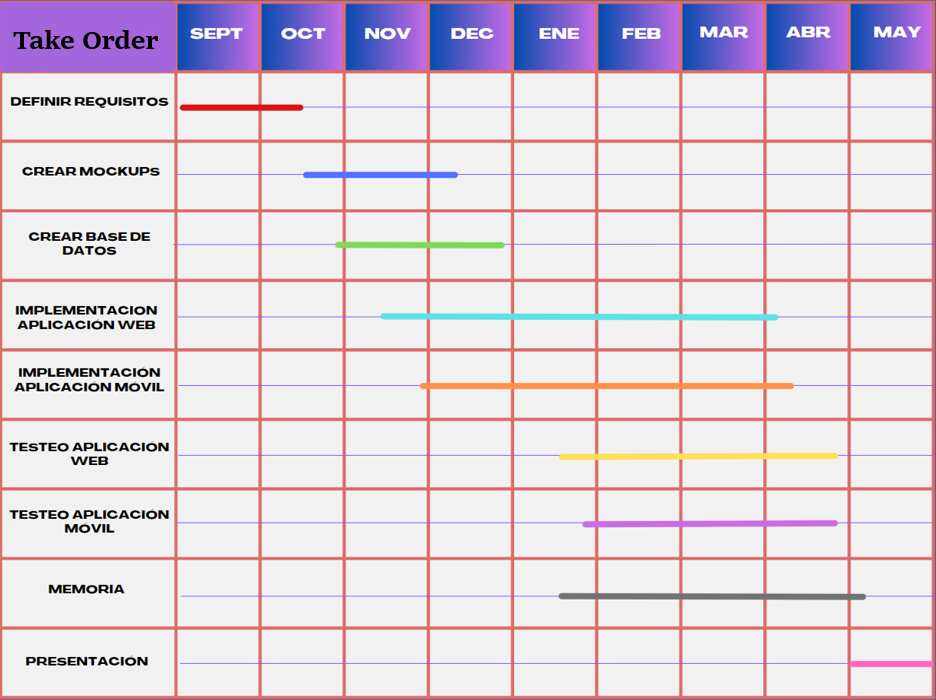
\includegraphics[width=15cm, height=11cm]{Imagenes/Figuras/Diagrama de Gantt.png}
\caption{Plan de proyecto}\label{fig:Diagrama de Gantt}
\end{figure} 


\begin{figure}[h]
\centering
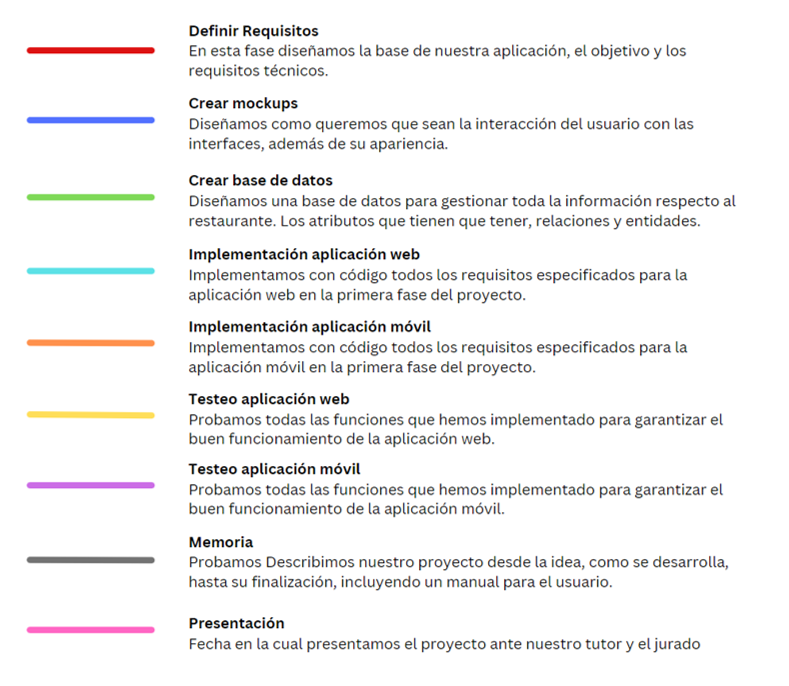
\includegraphics[width=15cm, height=12cm]{Imagenes/Figuras/leyenda Gantt.png}
\caption{Leyenda del plan de proyecto}\label{fig:Leyenda diagrama de Gantt}
\end{figure} 


\include{Capitulos/EstadoDeLaCuestion}
\include{Capitulos/AnálisisDeRequisitos}
\chapter{Entornos de Desarrollo}
\label{cap:EntornosDeDesarrollo}
\graphicspath{ {Imagenes/Figuras/} }


En este capítulo se van a enumerar una serie de librerías, herramientas, entornos y lenguajes
de programación que hemos utilizado y han facilitado la realización del proyecto.
También se procederá a explicar nuestro sistema de control de versiones y la base de datos empleada, además de las utilidades para prototipo de las interfaces.

\section{Frameworks y Librerías}
En esta sección se enumera la lista de entornos usados para el desarrollo de las dos aplicaciones, así como los \textit{frameworks} que nos han ayudado en la implementación del código.

\subsection{Visual Studio Code}

Visual Studio Code~\citep{VSCode} es un editor de código fuente desarrollado por Microsoft. Es un software libre y multiplataforma, que está disponible para Windows, GNU/Linux y macOS. VS Code tiene una buena integración con Git, cuenta con soporte para depuración de código, y dispone de un sin número de extensiones, que básicamente da la posibilidad de escribir y ejecutar código en cualquier lenguaje de programación.

\subsection{Android Studio}
Android Studio~\citep{AndroidStudio}, es el entorno de desarrollo integrado oficial del sistema operativo Android de Google, basado en el software IntelliJ IDEA de JetBrains y diseñado específicamente para el desarrollo de Android. Está disponible para su descarga en sistemas operativos basados en Windows, macOS y Linux. Además es el principal entorno de desarrollo para aplicaciones
móviles, con soporte para diversos lenguajes de programación como Java,
C++ y Kotlin.

\subsection{Maven}

Maven~\citep{Maven} es un \textit{Project Management Framework}, esto es, un \textit{framework} de gestión de proyectos de \textit{software}, que proporciona un modelo estándar de gestión y descripción de proyectos. Maven da soluciones a tareas que abarcan desde la compilación hasta la distribución, despliegue y documentación de los proyectos.

\subsection{Bootstrap}

Bootstrap~\citep{bootstrap} es un \textit{framework} CSS gratuito y de código abierto orientado al desarrollo web \textit{front-end} responsivo y \textit{mobile-first}. Contiene plantillas de diseño basadas en HTML, CSS y JavaScript para tipografía, formularios, botones, navegación y otros componentes de la interfaz.

\subsection{SweetAlert}

SweetAlert~\citep{sweetAlert} es una variante atractiva y muy personalizable para gestionar los \textit{pop-ups} emergentes en javascript.

\subsection{Docker}

Docker~\citep{docker} es un proyecto de código abierto que automatiza el despliegue de aplicaciones dentro de contenedores de software, proporcionando una capa adicional de abstracción y automatización de virtualización de aplicaciones en múltiples sistemas operativos.

\subsection{Fly.io}

Fly.io~\citep{fly.io} es una nueva nube pública, construida sobre servidores \textit{Bare-Metal} que se gestiona en centros de datos de todo el mundo, diseñada para facilitar el despliegue de aplicaciones distribuidas y en tiempo real cerca de sus usuarios, estén donde estén.

\section{Lenguajes de Programación}
Durante la realización del proyecto se han utilizado los lenguajes de programación presentados a continuación.

\subsection{HTML}

HTML~\citep{html} es el lenguaje de marcado estándar para documentos diseñados para visualizarse en un navegador web. Suele estar asistido por tecnologías como las hojas de estilo en cascada \textit{(Cascading Style Sheets)} y lenguajes de script como JavaScript.

\subsection{CSS}

CSS~\citep{css} es un lenguaje que permite el desarrollo del estilo de una página web cuando es utilizado sobre otro lenguaje de marcado, como en este caso HTML. Aunque la mayor parte del aspecto visual de la aplicación está realizado a través de Bootstrap se han incluido algunas hojas de estilo para añadir detalles que este \textit{framework} no contempla.

\subsection{Javascript}

JavaScript~\citep{javascript} es un lenguaje de programación que se utiliza para hacer páginas web interactivas. Desde actualizar fuentes de redes sociales a mostrar animaciones y mapas interactivos, las funciones de JavaScript pueden mejorar la experiencia del usuario de un sitio web.

\subsection{Java}

Java~\citep{java} es un lenguaje de programación ampliamente utilizado para codificar aplicaciones web. Ha sido una opción popular entre los desarrolladores durante más de dos décadas, con millones de aplicaciones Java en uso en la actualidad.

\subsection{Kotlin}

Kotlin~\citep{kotlin} es un lenguaje de programación de código abierto creado por JetBrains que se ha popularizado gracias a que se puede utilizar para programar aplicaciones Android.

\section{Bases de Datos}

Como gestor de base de datos decidimos usar \textit{Firebase} debido a su comodidad para integrarse en aplicaciones móviles realizadas con Android Studio.


Cloud Firestore~\citep{firestore} es una base de datos NoSQL orientada a documentos. A diferencia de una base de datos SQL, no hay tablas. En su lugar, se almacenan los datos en documentos, que se organizan en colecciones. Cada documento contiene un conjunto de pares clave-valor. En la Figura~\ref{fig:erd} podemos observar el diagrama entidad-relación

\begin{figure}[h]
\centering
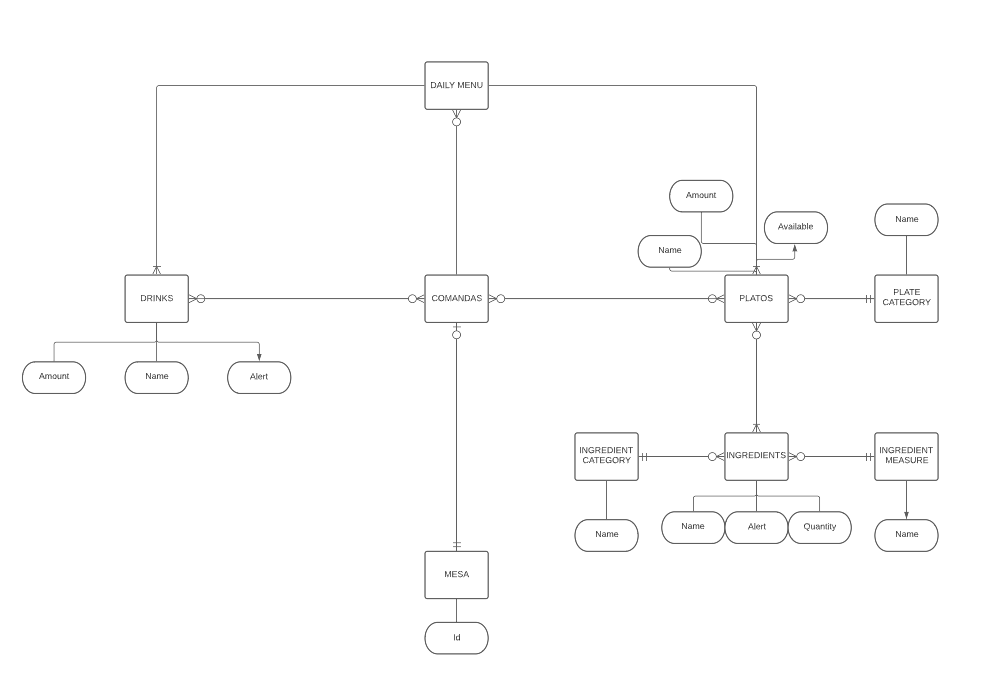
\includegraphics[width=16cm, height=13cm]{Imagenes/Figuras/ERD.png}
\caption{Diagrama entidad relación}\label{fig:erd}
\end{figure} 


\section{Control de Versiones}

GitHub~\citep{github} ofrece un servicio, tanto gratuito como de pago, para el control de versiones de proyectos usando la tecnología Git, registrando cada cambio subido al servidor gracias a su almacenamiento en la nube, y permitiendo volver a versiones anteriores o comparar los cambios realizados entre las mismas.
Decidimos usar esta plataforma dada nuestra experiencia con ella y que nos viene muy bien para trabajar paralelamente los proyectos.
Para ello creamos dos repositorios, uno para el desarrollo de la aplicación móvil, Figura~\ref{fig:githubapp}, y otro para el de la web, Figura~\ref{fig:githubweb}.

\begin{itemize}

\item Aplicación movil: 
\url{https://github.com/jesusmoraleda/TakeOrder.git}. 

\begin{figure}[h]
\centering
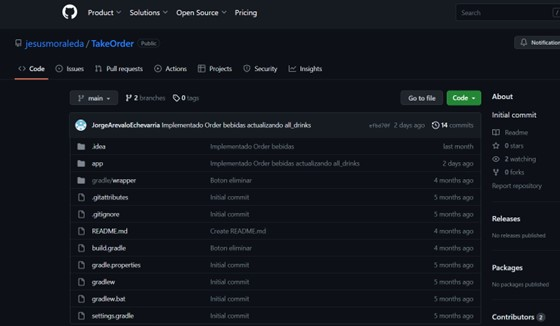
\includegraphics[width=13cm, height=8cm]{Imagenes/Figuras/GitHubAppMovil.jpg}
\caption{Repositorio del código de la aplicación}\label{fig:githubapp}
\end{figure} 



\item Aplicación web: 
\url{https://github.com/jesusmoraleda/TakeOrderAdmin.git}. 

\end{itemize}


\begin{figure}[h]
\centering
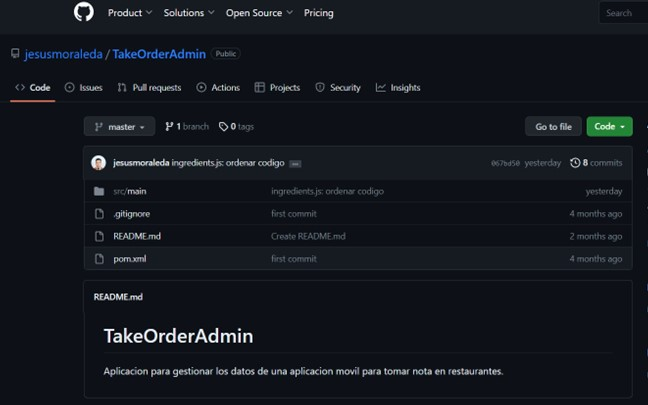
\includegraphics[width=13cm, height=8cm]{Imagenes/Figuras/GitHubAppWeb.jpg}
\caption{Repositorio del código web}\label{fig:githubweb}
\end{figure} 


\section{Maquetación y Prototipos}
Comenzamos desarrollando unos \textit{mockups} para que nos ayudaran a tener una idea general del aspecto que queríamos para la app móvil, como las que aparecen en las Figuras~\ref{fig:mockup1} y~\ref{fig:mockup2}, y para aplicación web como se puede visualizar en la Figura~\ref{fig:mockupWeb}, con el objetivo de resultar amistosa para el usuario.


\begin{figure}[h]
 \centering
  \subfloat[Mockup 1]{\label{fig:mockup1}
   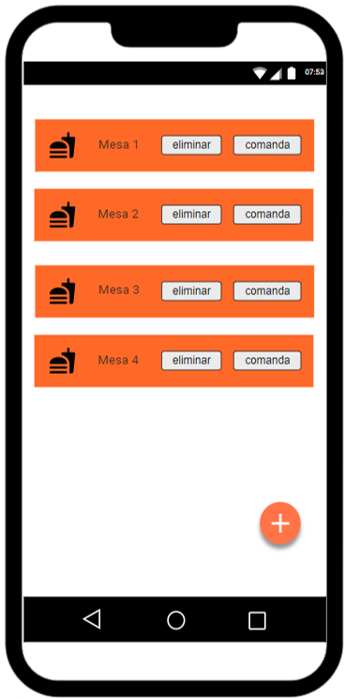
\includegraphics[width=4cm, height=8cm]{Imagenes/Figuras/mockup1.png}}
    \hfill
  \subfloat[Mockup 2]{\label{fig:mockup2}
    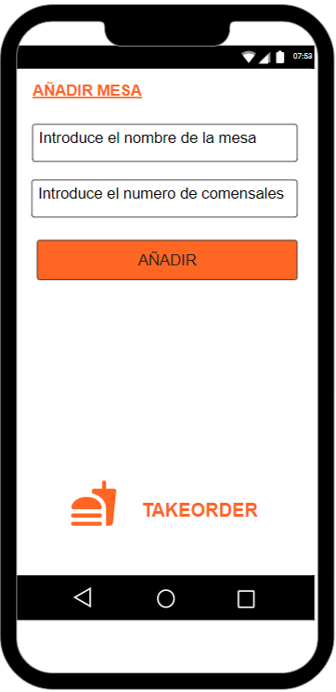
\includegraphics[width=4cm, height=8cm]{Imagenes/Figuras/mockup2.png}}
 \caption{Mockup aplicación Móvil}
\label{fig:mockupAppMovil}
\end{figure}

\begin{figure}[h]
 \centering
\scalebox{0.75}{ 
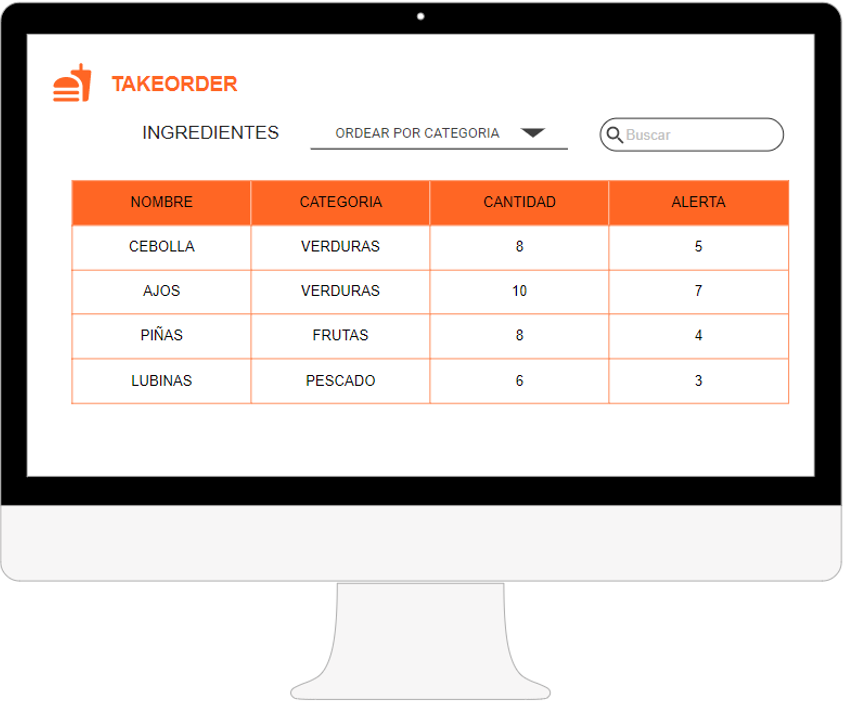
\includegraphics[width=11cm, height=9cm]{Imagenes/Figuras/mockupWeb.png}}
\caption{Mockup aplicación web}\label{fig:mockupWeb}
\end{figure} 



\include{Capitulos/Diseño-Implementacion.tex}
\chapter{Conclusiones y Trabajo Futuro}
\label{cap:conclusiones}

Una vez finalizado el proyecto, podemos decir que el objetivo de crear una aplicación para el mantenimiento del \textit{stock} de restaurantes se ha cumplido. Se ha quedado una interfaz muy intuitiva y sencilla de utilizar, que era el objetivo principal. Los objetivos alcanzados han sido:

\begin{itemize} 

\item Creación de distintas vistas para gestionar el \textit{stock} de un restaurante desde la visión del propietario del local.

\item Diseño de una base de datos para almacenar los ingredientes, bebidas y platos donde poder acceder y seleccionar la información.

\item Implementación de la aplicación móvil para que se puedan tomar nota desde cada mesa y simultáneamente se actualice el \textit{stock} del restaurante.

\item Implementación de la aplicación web para poder gestionar el \textit{stock} de los ingredientes, bebidas y platos del restaurante y se actualice la base de datos al momento.
 
\item Diseñar un aspecto visual agradable que haga una mejor experiencia del usuario, tanto en la aplicación web como en la aplicación móvil.

 \end{itemize}

Todas las funcionalidades se han desarrollado de manera independiente, tratando de tener un código limpio y organizado, lo que nos permitirá añadir nuevas funcionalidades de manera cómoda y sencilla.

En cuanto a la funcionalidad de las aplicaciones, se han solventado los requisitos mínimos para poder gestionar un restaurante, pero es fácil añadir nuevas características que sean requeridas en cada establecimiento en particular.

Como trabajo futuro nos gustaría enumerar una serie de ideas que se podrían implementar:
\begin{itemize}

 \item \textbf{Limitaciones de Firebase}. Se ha usado Firebase para la implementación, ya que es una base de datos muy práctica para proyectos pequeños. 
Sin embargo, se ha usado un plan de datos gratuito, el cual tiene límite de consultas y de usuarios simultáneos. Para implementarlo en un restaurante se debería pasar a un plan de pago. Si se quiere usar para grandes cadenas de restaurantes, por ejemplo, habría que estudiar el rendimiento y la posibilidad de cambiar a otra base de datos

\item \textbf{Mejoras en el dominio}. Al igual que en la base de datos, se ha usado una página web que nos ofrece un dominio por tiempo limitado. Habría que estudiar la posibilidad de comprar y hacernos con el dominio \textit{TakeOrderAdmin.es.}

\item \textbf{Alertas.}
Se podría añadir una funcionalidad para notificar mediante un email al encargado del \textit{stock} de las alertas asociadas a los ingredientes y bebidas.

\item \textbf{Precio y proveedores.}
Implementar campos para guardar los precios y los proveedores de los ingredientes y bebidas sería muy útil.

\item \textbf{Menús del día.}
Sería interesante tener una serie de menús del día ya predefinidos, por ejemplo para cada día de la semana, y poder cargarlos rápidamente.

También se podría añadir una funcionalidad para poder acceder a estos menús del día o a toda la carta mediante un código QR o poder imprimirlos con un formato adecuado.

\item \textbf{Creación de usuarios}.
Se podrían integrar la creación usuarios, de tal forma que podamos restringir algunas funcionalidades a ciertos trabajadores, o poder mostrar alguna información sensible como precios y proveedores solo al administrador del \textit{stock}.
\end{itemize}



%%%%%%%%%%%%%%%%%%%%%%%%%%%%%%%%%%%%%%%%%%%%%%%%%%%%%%%%%%%%%%%%%%%%%%%%%%%
% Si el TFG se escribe en inglés, comentar las siguientes líneas 
% porque no es necesario incluir nuevamente las Conclusiones en inglés
\begin{otherlanguage}{english}
\chapter*{Introduction}
\label{cap:introduction}
\addcontentsline{toc}{chapter}{Introduction}

This document contains all the fundamental aspects to understand the functionality of the web and mobile application designed as a Final Degree Project to facilitate the management of ingredients stock in restaurants.

The idea of the project comes from the need of a fast and efficient management when managing a restaurant, which are some of the most important qualities to achieve a successful business.

Until recently, in any restaurant, the way of carrying out the work was based on the waiter taking note of what the customer wanted with a notebook and pen, and take it to the kitchen for preparation. Even the waiter could even say the typical expression: "I'm going to check with the kitchen to see if that plate is available", although we can still see this type of management nowadays in any town or beach bar.

We are in a new digital era in which we need tools to facilitate our work, with the quality that our clients expect. The idea, therefore, is to accelerate as much as possible the organizational processes of a restaurant, so that the restaurant manager can plan and structure the service to customers, having access to the design configuration of the menu of the day, and the plates to be prepared.

In the world of gastronomy, success is based on good raw materials, a good preparation of the plates and an excellent customer service with a fast and quality service. In our case, we have focused on this last point, reducing time-consuming manual tasks that make it more difficult to concentrate on customer service with a quality service.

To achieve this objective, our project focuses, on the one hand, on a dynamic communication between kitchen and dining room employees, providing a fast and efficient management when serving customers and, on the other hand, on facilitating a simple administration management of the stock of ingredients and products.


\section{Objetives}

The software developed is focused on improving and optimizing stock management and communication between waiters and the kitchen. The objectives will be, therefore, the efficiency improvement, reduction of the time required and increase of the quality of service to customers with an automated task system combined with an extensive database  where all information can be stored and accessed quickly.

The use of a web application for the management and administration of the restaurant ensures that the plates, drinks or menus available are exactly the same as the offered to the customer and that there are no errors between the cooks and the waiters. Immediate access to the database information is allowed in order to manage the restaurant's stock. Stock updating will be extremely simple, as the manager will only have to replenishment the ingredients that are below the minimum levels, for which an alert is generated. This will give the manager an idea for which plates to include in that daily menu.

From the point of view of the employee, in this case the waiters, the use of a mobile application for internal communication between employees ensures direct communication with the customer by offering and informing them of the products available in both plates and drinks. This generates a fast and quality service when managing the orders for each table, without generating waits or questions in the kitchen that may upset the customer.

From the technological point of view, the objectives of this project are as follows:

\begin{itemize}

\item For the web application, design a software with a simple interface that facilitates the work of the application manager, such as seeing the ingredients that have generated an alert for being below minimum stock levels for a replenishment of those ingredients. In addition, you will be able to generate a
menu of the day, being able to select the number of plates to be prepared for that day, based on the available ingredients, managing which plates will be offered as first course, second course and dessert.

\item For the mobile application, design in the same way a simple  interface that facilitates the work of the restaurant workers, both waiters and cooks. They will be able to generate an order assigned to a table being able to take note of the drinks and the plates offered by the menu, in addition to offer a menu of the day taking note of the first and second plates, and the dessert.

\item Design a database that allows the storage of a large amount of information, in which we will store all the ingredients registered in the restaurant, the plates with their assigned ingredients, the drinks or the tables, each one assigned with an order, and in each order, stored the plates and drinks ordered by that table.

\end{itemize}


\section{Work plan}

Considering the objectives described above, a time estimate was made for the work plan with a duration of 7 months. In order to be able to see the work plan in a clear and simple way we decided to make a Gantt diagram.
We can see work plan in the Figure~\ref{fig:Diagrama de Gantt(ingles)} and description of the activities in the Figure~\ref{fig:Leyenda diagrama de Gantt(ingles)}

\begin{figure}[h]
\centering
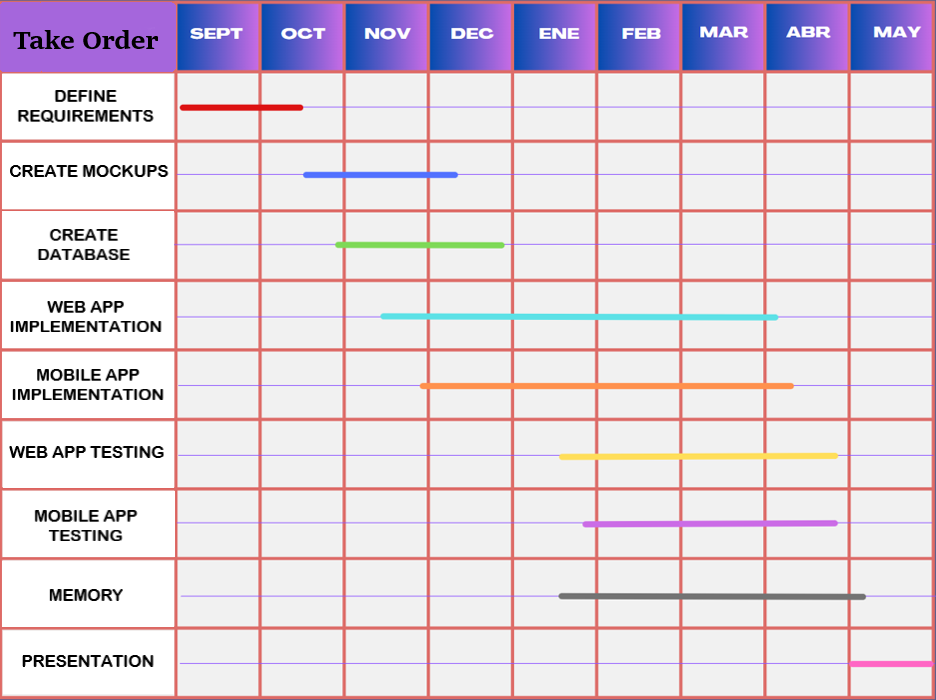
\includegraphics[width=15cm, height=11cm]{Imagenes/Figuras/Diagrama de Gantt (ingles).png}
\caption{Work plan}\label{fig:Diagrama de Gantt(ingles)}
\end{figure} 


\begin{figure}[h]
\centering
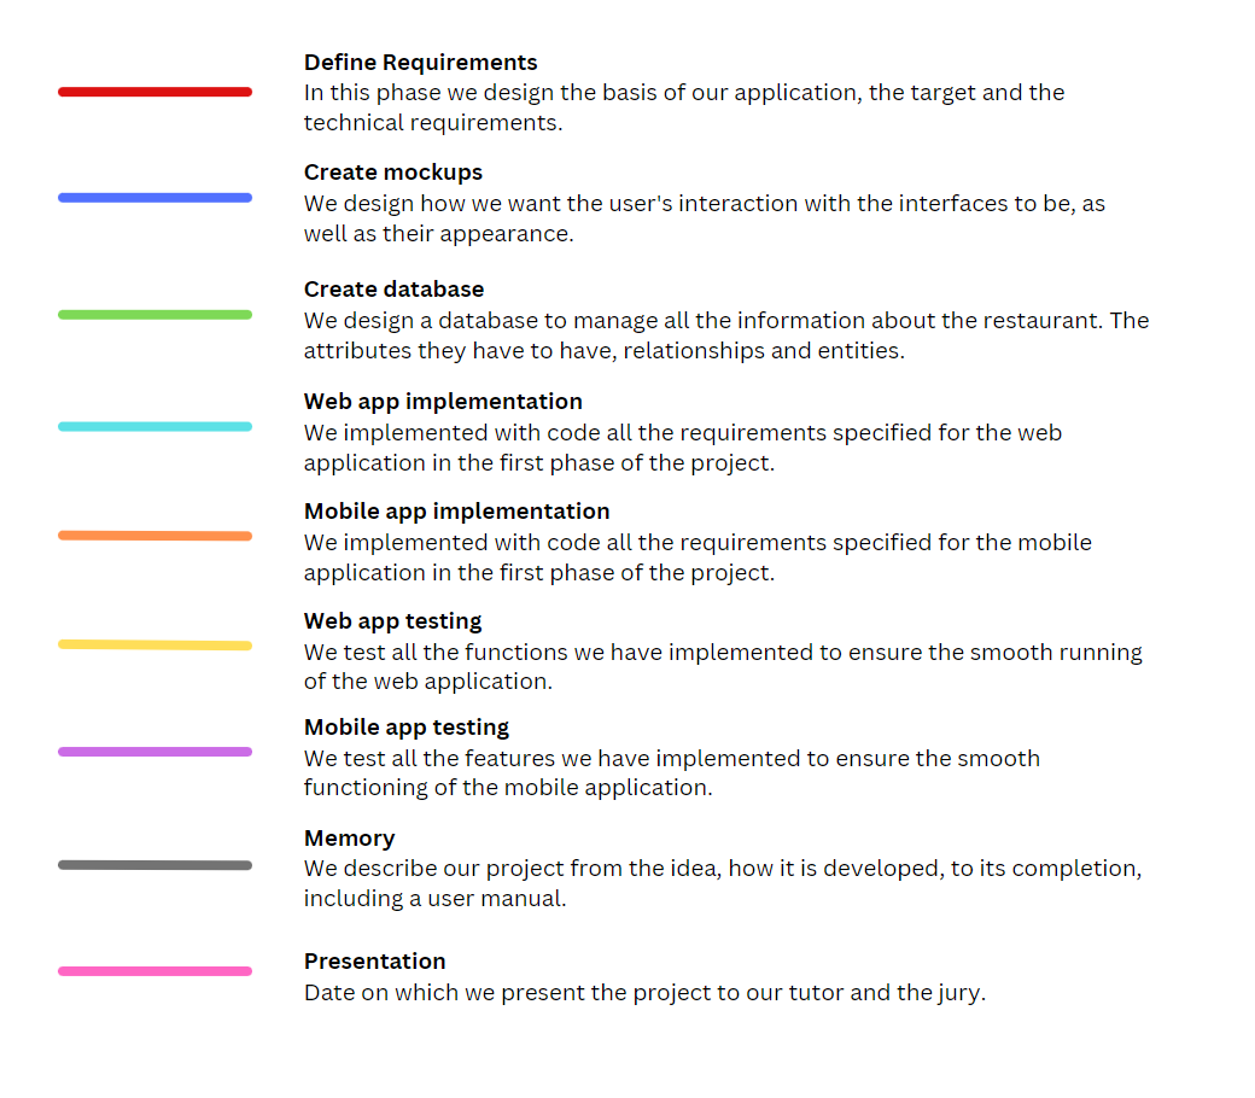
\includegraphics[width=15cm, height=12cm]{Imagenes/Figuras/leyenda Gantt (ingles).png}
\caption{Work plan legend}\label{fig:Leyenda diagrama de Gantt(ingles)}
\end{figure} 








\chapter*{Conclusions and Future Work}
\label{cap:conclusions}
\addcontentsline{toc}{chapter}{Conclusions and Future Work}

Once the project is finished, we can say that the objective of creating an application for the maintenance of restaurants has been achieved. It has resulted in a very intuitive and easy to use interface, which was the main objective. Some of the objectives have been achieved:

\begin{itemize} 

\item Creation of different views to manage the stock of a restaurant from the owner's point of view.
 
\item Design of a database to store the ingredients, drinks and plates where the information can be accessed and selected.

\item Implementation of the mobile app so that waiters can take notes from each table and simultaneously update the restaurant's stock.

\item Design a friendly visual appearance that makes a better user experience, both in the web application and in the mobile application.

 \end{itemize}

All the functionalities have been developed independently, trying to have a clean and organized code, which will allow us to add new functionalities in a comfortable and simple way.

As for the functionality of the applications, the minimum requirements to manage a restaurant have been solved, but it is easy to add new features that are required in each particular establishment.

As future work we would like to list a number of ideas that could be implemented:
\begin{itemize}

\item \textbf{Firebase Limitations}
Firebase has been used for the implementation as it is a very practical database for small projects. 
First of all a free data plan has been used, which has a limit of queries and simultaneous users, to implement it in a restaurant it would be necessary to change to a paid plan, if you want to use it for large restaurant chains, for example, you would have to study the performance and the possibility of changing to another database.

 \item \textbf{Domain improvements}
As in the database, we have used a web domain that offers us a domain for a limited time. It would be necessary to study the possibility of buying and getting the domain TakeOrderAdmin.es 

 \item \textbf{Alerts}
It would be possible to add a funcionality to notify by email to he owner of the restaurant when there is some ingredient or drink in alert.

 \item \textbf{Price and providers}
Implementing fields to store prices and providers of ingredients and drinks would be very useful.

 \item \textbf{Menus of the day}
It would be interesting to have a predefined set of menus of the day for example for each day of the week, and to be able to load them quickly.

You could also add a functionality to access these menus of the day or the entire menu via a QR code or to print them in a suitable format.

\item \textbf{User creation}
The creation of users could be created, so that we can restrict some functionalities to certain workers, or be able to show some sensitive information like prices and suppliers only to the restaurant owner.  \ref{cap:conclusiones}.

\end{itemize}


\end{otherlanguage}
%%%%%%%%%%%%%%%%%%%%%%%%%%%%%%%%%%%%%%%%%%%%%%%%%%%%%%%%%%%%%%%%%%%%%%%%%%%

\chapter*{Contribuciones Personales}
\label{cap:contribucionesPersonales}
\addcontentsline{toc}{chapter}{Contribuciones Personales}

Desde un inicio decidimos repartirnos el trabajo de manera que los dos tuviéramos la misma carga. Nos hemos compenetrado muy bien fortaleciendo los puntos fuertes de cada uno. Aunque se ha dividido el trabajo de desarrollo de las aplicaciones, hemos estado siempre en contacto, consultándonos dudas y proponiendo nuevas ideas el uno al otro.


\section*{Jesús Martín Moraleda}
Al principio del proyecto, consideramos invertir un tiempo en estudiar todas las tecnologías que podíamos utilizar, ya que el desarrollo web y móvil era prácticamente nuevo para nosotros. Me encargué de probar e informarme de ventajas e inconvenientes de cada una y decidir las que íbamos a usar.
Del mismo modo investigué que base de datos nos convenía usar y como conectar nuestras aplicaciones con esta.

Una vez teníamos claras las tecnologías, me dediqué a crear el proyecto de la base de datos en \textit{Firebase} y, junto a Jorge, a conectar las aplicaciones con la base de datos. Una vez las dos aplicaciones se comunicaban correctamente con la base de datos, me encargué de crear un repositorio de GitHub para cada proyecto. Una vez hice los primeros \textit{commits} con la estructura del proyecto y la conexión con la base de datos, Jorge empezó con el desarrollo de la aplicación móvil y yo me dediqué al desarrollo de la web.

Con todo esto listo, empecé con el desarrollo de la página web con la ayuda de los \textit{mockups} que había realizado mi compañero. Empecé desarrollando la pantalla de los ingredientes. Mi objetivo era ir desarrollando las vistas completas y que funcionaran correctamente. Luego seguí con las pantallas de bebidas e ingredientes, y mas tarde realice las vistas del menú del día y las alertas.

Mientras hacíamos todo esto, teníamos reuniones con Mercedes, que nos fue guiando en el desarrollo del proyecto. Nos dió libertad para usar las tecnologías que quisieramos, y las funcionalidades de la aplicación las debatíamos entre los tres en estas reuniones.

En mitad del desarrollo, me puse a investigar como podíamos desplegar la página web en un dominio, para que se pudiera acceder de otra manera que desde nuestros ordenadores. Esto me llevó un tiempo ya que no habíamos tenido que desplegar una página web anteriormente.

En esta fase de desarrollo, Jorge y yo debatíamos juntos las dudas y las cosas nuevas que queríamos implementar en las dos aplicaciones. Veíamos como poder implementarlas y que tuvieran concordancia las funcionalidades de una aplicación con la otra.

La memoria la fuimos completando a medida que íbamos avanzando en las fases. Mercedes nos fue ayudando a como estructurarla e implementarla

\section*{Jorge Arévalo Echevarría}

Durante la fase de análisis realizábamos reuniones con nuestra tutora, para ir dando forma y moldeando en que dirección queríamos llevar el proyecto, definiendo los requisitos y las funcionalidades que queríamos llevar a cabo. Nuestra tutora nos dio completa libertad para la selección de entornos de desarrollo o lenguajes de programación, dejándonos escoger con los que nos sintiésemos más cómodos. Además, hicimos un diseño previo de como sería nuestra base de datos que se encargaría de almacenar la información de nuestras aplicaciones. Así que por último empezamos a planificar y dividir el trabajo para investigar que entornos utilizar para el proyecto.

Durante la fase de investigación mi labor consistió en el estudio y diseño de la base de datos y de la aplicación móvil.

Respecto a la base de datos, empecé investigando los entorno conocidos y utilizados en las distintas asignaturas de la carrera como "Bases de Datos" en la que utilizábamos el entorno Oracle Database. Después vimos que era muy buen entorno para desarrollar la base de datos a nuestro gusto, pero nos surgió el problema de que los ejemplos que estábamos acostumbrados a hacer en clase trabajábamos en local, y nosotros necesitábamos una base de datos remota para poder acceder a los datos desde la página web. Jesús me informo sobre "Firestone Firebase" siendo muy fácil e intuitivo para proyectos a pequeña escala, teniendo un gran resultado en el desarrollo de sus proyectos, además de ser un entorno gratuito. Así, Jesús se encargó del diseño e instalación de la base de datos para el desarrollo de nuestro proyecto.

Respecto a la aplicación móvil, yo ya tenía experiencia respecto a entornos de desarrollo, ya que utilice Android Studio en la asignatura optativa de "Programación de aplicaciones para dispositivos móviles". Lo que más me gusto fue la libertad que proporciona a la hora de diseñar las vistas, además de usar el lenguaje de programación Java, con el que todos estamos familiarizados. Respecto a las vistas para la aplicación móvil, decidimos realizar unos \textit{mockups} para ir diseñando y plasmando las ideas preconcebidas que teníamos en la cabeza, de como queríamos que fuese la aplicación y que funcionalidades queríamos que llevase a cabo.

En la fase de configuración y de instalación, me encargué de la instalación de la última versión de Android Studio en nuestros dispositivos. También generamos un repositorio en Github para comprobar las actualizaciones realizadas, además de controlar y guardar las versiones anteriores de nuestro proyecto de la aplicación móvil.

La fase de desarrollo se puede decir que fue la más compleja de las fases, ya que fue la que nos llevó más tiempo y esfuerzo. Durante esta fase me encargué de llevar a cabo la implementación de las ideas que habíamos preconcebido para la aplicación móvil. Lo primero que hice fue enlazar mi proyecto al repositorio de Github, para poder controlar la subida y actualizaciones del proyecto, o en caso de cometer un error, poder recuperar una versión que funcionase de forma correcta.
Después, uno de los pasos más importantes fue el de realizar la conexión del proyecto con la base de datos Firestore database, para poder obtener la información o editar campos dentro de la base de datos. A partir de aquí desarrollé todas las vistas y funcionalidades de la aplicación móvil, en colaboración con Jesús, mientras desarrollaba la página web, para ir dando forma al producto final que queríamos obtener.

La memoria del proyecto la fuimos completando mientras íbamos avanzando en las distintas fases del proyecto. Gracias a la corrección y supervisión de nuestra tutora que nos daba indicaciones de qué partes debíamos modificar o mejorar, encarrilando y dirigiendo la memoria para conseguir un nivel apto de entrega. 





%
% Bibliografía
%
% Si el TFM se escribe en inglés, editar TeXiS/TeXiS_bib para cambiar el
% estilo de las referencias
%---------------------------------------------------------------------
%
%                      configBibliografia.tex
%
%---------------------------------------------------------------------
%
% bibliografia.tex
% Copyright 2009 Marco Antonio Gomez-Martin, Pedro Pablo Gomez-Martin
%
% This file belongs to the TeXiS manual, a LaTeX template for writting
% Thesis and other documents. The complete last TeXiS package can
% be obtained from http://gaia.fdi.ucm.es/projects/texis/
%
% Although the TeXiS template itself is distributed under the 
% conditions of the LaTeX Project Public License
% (http://www.latex-project.org/lppl.txt), the manual content
% uses the CC-BY-SA license that stays that you are free:
%
%    - to share & to copy, distribute and transmit the work
%    - to remix and to adapt the work
%
% under the following conditions:
%
%    - Attribution: you must attribute the work in the manner
%      specified by the author or licensor (but not in any way that
%      suggests that they endorse you or your use of the work).
%    - Share Alike: if you alter, transform, or build upon this
%      work, you may distribute the resulting work only under the
%      same, similar or a compatible license.
%
% The complete license is available in
% http://creativecommons.org/licenses/by-sa/3.0/legalcode
%
%---------------------------------------------------------------------
%
% Fichero  que  configura  los  parámetros  de  la  generación  de  la
% bibliografía.  Existen dos  parámetros configurables:  los ficheros
% .bib que se utilizan y la frase célebre que aparece justo antes de la
% primera referencia.
%
%---------------------------------------------------------------------


%%%%%%%%%%%%%%%%%%%%%%%%%%%%%%%%%%%%%%%%%%%%%%%%%%%%%%%%%%%%%%%%%%%%%%
% Definición de los ficheros .bib utilizados:
% \setBibFiles{<lista ficheros sin extension, separados por comas>}
% Nota:
% Es IMPORTANTE que los ficheros estén en la misma línea que
% el comando \setBibFiles. Si se desea utilizar varias líneas,
% terminarlas con una apertura de comentario.
%%%%%%%%%%%%%%%%%%%%%%%%%%%%%%%%%%%%%%%%%%%%%%%%%%%%%%%%%%%%%%%%%%%%%%
\setBibFiles{%
biblio%
}

%%%%%%%%%%%%%%%%%%%%%%%%%%%%%%%%%%%%%%%%%%%%%%%%%%%%%%%%%%%%%%%%%%%%%%
% Definición de la frase célebre para el capítulo de la
% bibliografía. Dentro normalmente se querrá hacer uso del entorno
% \begin{FraseCelebre}, que contendrá a su vez otros dos entornos,
% un \begin{Frase} y un \begin{Fuente}.
%
% Nota:
% Si no se quiere cita, se puede eliminar su definición (en la
% macro setCitaBibliografia{} ).
%%%%%%%%%%%%%%%%%%%%%%%%%%%%%%%%%%%%%%%%%%%%%%%%%%%%%%%%%%%%%%%%%%%%%%
\setCitaBibliografia{
\begin{FraseCelebre}
\begin{Frase}
  Y así, del mucho leer y del poco dormir, se le secó el celebro de
  manera que vino a perder el juicio.
\end{Frase}
\begin{Fuente}
  Miguel de Cervantes Saavedra
\end{Fuente}
\end{FraseCelebre}
}

%%
%% Creamos la bibliografia
%%
\makeBib

% Variable local para emacs, para  que encuentre el fichero maestro de
% compilación y funcionen mejor algunas teclas rápidas de AucTeX

%%%
%%% Local Variables:
%%% mode: latex
%%% TeX-master: "../Tesis.tex"
%%% End:



% Apéndices
\appendix
%\chapter{Título del Apéndice A}
\label{Appendix:Key1}

Los apéndices son secciones al final del documento en las que se agrega texto con el objetivo de ampliar los contenidos del documento principal.
%\chapter{Título del Apéndice B}
\label{Appendix:Key2}

Se pueden añadir los apéndices que se consideren oportunos.
%\include{Apendices/appendixC}
%\include{...}
%\include{...}
%\include{...}
\backmatter



%
% Índice de palabras
%

% Sólo  la   generamos  si  está   declarada  \generaindice.  Consulta
% TeXiS.sty para más información.

% En realidad, el soporte para la generación de índices de palabras
% en TeXiS no está documentada en el manual, porque no ha sido usada
% "en producción". Por tanto, el fichero que genera el índice
% *no* se incluye aquí (está comentado). Consulta la documentación
% en TeXiS_pream.tex para más información.
\ifx\generaindice\undefined
\else
%%---------------------------------------------------------------------
%
%                        TeXiS_indice.tex
%
%---------------------------------------------------------------------
%
% TeXiS_indice.tex
% Copyright 2009 Marco Antonio Gomez-Martin, Pedro Pablo Gomez-Martin
%
% This file belongs to TeXiS, a LaTeX template for writting
% Thesis and other documents. The complete last TeXiS package can
% be obtained from http://gaia.fdi.ucm.es/projects/texis/
%
% This work may be distributed and/or modified under the
% conditions of the LaTeX Project Public License, either version 1.3
% of this license or (at your option) any later version.
% The latest version of this license is in
%   http://www.latex-project.org/lppl.txt
% and version 1.3 or later is part of all distributions of LaTeX
% version 2005/12/01 or later.
%
% This work has the LPPL maintenance status `maintained'.
% 
% The Current Maintainers of this work are Marco Antonio Gomez-Martin
% and Pedro Pablo Gomez-Martin
%
%---------------------------------------------------------------------
%
% Contiene  los  comandos  para  generar  el índice  de  palabras  del
% documento.
%
%---------------------------------------------------------------------
%
% NOTA IMPORTANTE: el  soporte en TeXiS para el  índice de palabras es
% embrionario, y  de hecho  ni siquiera se  describe en el  manual. Se
% proporciona  una infraestructura  básica (sin  terminar)  para ello,
% pero  no ha  sido usada  "en producción".  De hecho,  a pesar  de la
% existencia de  este fichero, *no* se incluye  en Tesis.tex. Consulta
% la documentación en TeXiS_pream.tex para más información.
%
%---------------------------------------------------------------------


% Si se  va a generar  la tabla de  contenidos (el índice  habitual) y
% también vamos a  generar el índice de palabras  (ambas decisiones se
% toman en  función de  la definición  o no de  un par  de constantes,
% puedes consultar modo.tex para más información), entonces metemos en
% la tabla de contenidos una  entrada para marcar la página donde está
% el índice de palabras.

\ifx\generatoc\undefined
\else
   \addcontentsline{toc}{chapter}{\indexname}
\fi


% Generamos el índice
\printindex

% Variable local para emacs, para  que encuentre el fichero maestro de
% compilación y funcionen mejor algunas teclas rápidas de AucTeX

%%%
%%% Local Variables:
%%% mode: latex
%%% TeX-master: "./tesis.tex"
%%% End:

\fi

%
% Lista de acrónimos
%

% Sólo  lo  generamos  si  está declarada  \generaacronimos.  Consulta
% TeXiS.sty para más información.


\ifx\generaacronimos\undefined
\else
%---------------------------------------------------------------------
%
%                        TeXiS_acron.tex
%
%---------------------------------------------------------------------
%
% TeXiS_acron.tex
% Copyright 2009 Marco Antonio Gomez-Martin, Pedro Pablo Gomez-Martin
%
% This file belongs to TeXiS, a LaTeX template for writting
% Thesis and other documents. The complete last TeXiS package can
% be obtained from http://gaia.fdi.ucm.es/projects/texis/
%
% This work may be distributed and/or modified under the
% conditions of the LaTeX Project Public License, either version 1.3
% of this license or (at your option) any later version.
% The latest version of this license is in
%   http://www.latex-project.org/lppl.txt
% and version 1.3 or later is part of all distributions of LaTeX
% version 2005/12/01 or later.
%
% This work has the LPPL maintenance status `maintained'.
% 
% The Current Maintainers of this work are Marco Antonio Gomez-Martin
% and Pedro Pablo Gomez-Martin
%
%---------------------------------------------------------------------
%
% Contiene  los  comandos  para  generar  el listado de acrónimos
% documento.
%
%---------------------------------------------------------------------
%
% NOTA IMPORTANTE:  para que la  generación de acrónimos  funcione, al
% menos  debe  existir  un  acrónimo   en  el  documento.  Si  no,  la
% compilación  del   fichero  LaTeX  falla  con   un  error  "extraño"
% (indicando  que  quizá  falte  un \item).   Consulta  el  comentario
% referente al paquete glosstex en TeXiS_pream.tex.
%
%---------------------------------------------------------------------


% Redefinimos a español  el título de la lista  de acrónimos (Babel no
% lo hace por nosotros esta vez)

\def\listacronymname{Lista de acrónimos}

% Para el glosario:
% \def\glosarryname{Glosario}

% Si se  va a generar  la tabla de  contenidos (el índice  habitual) y
% también vamos a  generar la lista de acrónimos  (ambas decisiones se
% toman en  función de  la definición  o no de  un par  de constantes,
% puedes consultar config.tex  para más información), entonces metemos
% en la  tabla de contenidos una  entrada para marcar  la página donde
% está el índice de palabras.

\ifx\generatoc\undefined
\else
   \addcontentsline{toc}{chapter}{\listacronymname}
\fi


% Generamos la lista de acrónimos (en realidad el índice asociado a la
% lista "acr" de GlossTeX)

\printglosstex(acr)

% Variable local para emacs, para  que encuentre el fichero maestro de
% compilación y funcionen mejor algunas teclas rápidas de AucTeX

%%%
%%% Local Variables:
%%% mode: latex
%%% TeX-master: "../Tesis.tex"
%%% End:

\fi

%
% Final
%
%%---------------------------------------------------------------------
%
%                      fin.tex
%
%---------------------------------------------------------------------
%
% fin.tex
% Copyright 2009 Marco Antonio Gomez-Martin, Pedro Pablo Gomez-Martin
%
% This file belongs to the TeXiS manual, a LaTeX template for writting
% Thesis and other documents. The complete last TeXiS package can
% be obtained from http://gaia.fdi.ucm.es/projects/texis/
%
% Although the TeXiS template itself is distributed under the 
% conditions of the LaTeX Project Public License
% (http://www.latex-project.org/lppl.txt), the manual content
% uses the CC-BY-SA license that stays that you are free:
%
%    - to share & to copy, distribute and transmit the work
%    - to remix and to adapt the work
%
% under the following conditions:
%
%    - Attribution: you must attribute the work in the manner
%      specified by the author or licensor (but not in any way that
%      suggests that they endorse you or your use of the work).
%    - Share Alike: if you alter, transform, or build upon this
%      work, you may distribute the resulting work only under the
%      same, similar or a compatible license.
%
% The complete license is available in
% http://creativecommons.org/licenses/by-sa/3.0/legalcode
%
%---------------------------------------------------------------------
%
% Contiene la última página
%
%---------------------------------------------------------------------


% Ponemos el marcador en el PDF
\ifpdf
   \pdfbookmark{Fin}{fin}
\fi

\thispagestyle{empty}\mbox{}

Este texto se puede encontrar en el fichero Cascaras/fin.tex. Si deseas eliminarlo, basta con comentar la línea correspondiente al final del fichero TFGTeXiS.tex.

\vspace*{4cm}

\small

\hfill \emph{--¿Qué te parece desto, Sancho? -- Dijo Don Quijote --}

\hfill \emph{Bien podrán los encantadores quitarme la ventura,}

\hfill \emph{pero el esfuerzo y el ánimo, será imposible.}

\hfill 

\hfill \emph{Segunda parte del Ingenioso Caballero} 

\hfill \emph{Don Quijote de la Mancha}

\hfill \emph{Miguel de Cervantes}

\vfill%space*{4cm}

\hfill \emph{--Buena está -- dijo Sancho --; fírmela vuestra merced.}

\hfill \emph{--No es menester firmarla -- dijo Don Quijote--,}

\hfill \emph{sino solamente poner mi rúbrica.}

\hfill 

\hfill \emph{Primera parte del Ingenioso Caballero} 

\hfill \emph{Don Quijote de la Mancha}

\hfill \emph{Miguel de Cervantes}


\newpage
\thispagestyle{empty}\mbox{}

\newpage

% Variable local para emacs, para  que encuentre el fichero maestro de
% compilación y funcionen mejor algunas teclas rápidas de AucTeX

%%%
%%% Local Variables:
%%% mode: latex
%%% TeX-master: "../Tesis.tex"
%%% End:

%\end{otherlanguage}
\end{document}
